\documentclass[12pt]{article}

\bibliographystyle{unsrt}
\renewcommand\refname{Bibliografia}

\usepackage[utf8]{inputenc}
\usepackage{parskip}
\usepackage{graphicx}
\usepackage{tabularray}
\usepackage{pdflscape}
\usepackage{afterpage}
\usepackage{caption}
\usepackage{float}
\graphicspath{ {./images/} }
\setlength{\parindent}{0cm}

\begin{document}


\section{Classificação do Algodão}

O procedimento para a classificação da pluma do algodão é estabelecido pela Instrução Normativa n. 24 de 2016 do Ministério da Agricultura e leva em consideração Padrões Físicos Universais, como a cor da fibra, a presença de folhas e impurezas, contaminação de matérias estranhas e o modo de beneficionamento do produto \cite{2016in24}.

Tem início com o processo de amostragem, que leva em consideração os seguintes pontos:

\begin{itemize}
    \item A amostra pode ser realizada manualmente ou mecanicamente;
    \item De cada fardo deve-se extrair duas amostras de lados opostos (no mínimo 150 gramas cada). Cada uma dessas amostras será dividida no sentido longitudinal e essa metada adicionada à medade da outra amostra, formando assim duas amostras de trabalho. Uma será enviada para classificação visual e outra para classificação tecnológica;
    \item As amostras devem ser manuseadas e acondicionadas em pacotes de forma a não descaracterizá-las ao longo do processo;
    \item O tamanho das amostras deve ter no mínimo 25 a 30 centímetros de comprimento, 13 a 15 centímetros de largura e 8 a 13 centímetros de espessura;
\end{itemize}

Após, as amostras retiradas seguem para o processo de classificação visual. Neste processo é utilizado como referência os Padrões Físicos Universais, que consistem em caixas com 6 amostras de algodão, tendo como base os padrões americanos para os algodões "\textit{Upland}" e "\textit{Pima}", conforme exemplo na Figura \ref{fig_padrao_fisico}.

\begin{figure}[H]
	\caption{\label{fig_padrao_fisico} Exemplo do Padrão Físico Universal (51.5: Cor Abaixo da Média, Branco / Grau de Folhas 5)}
	\begin{center}
		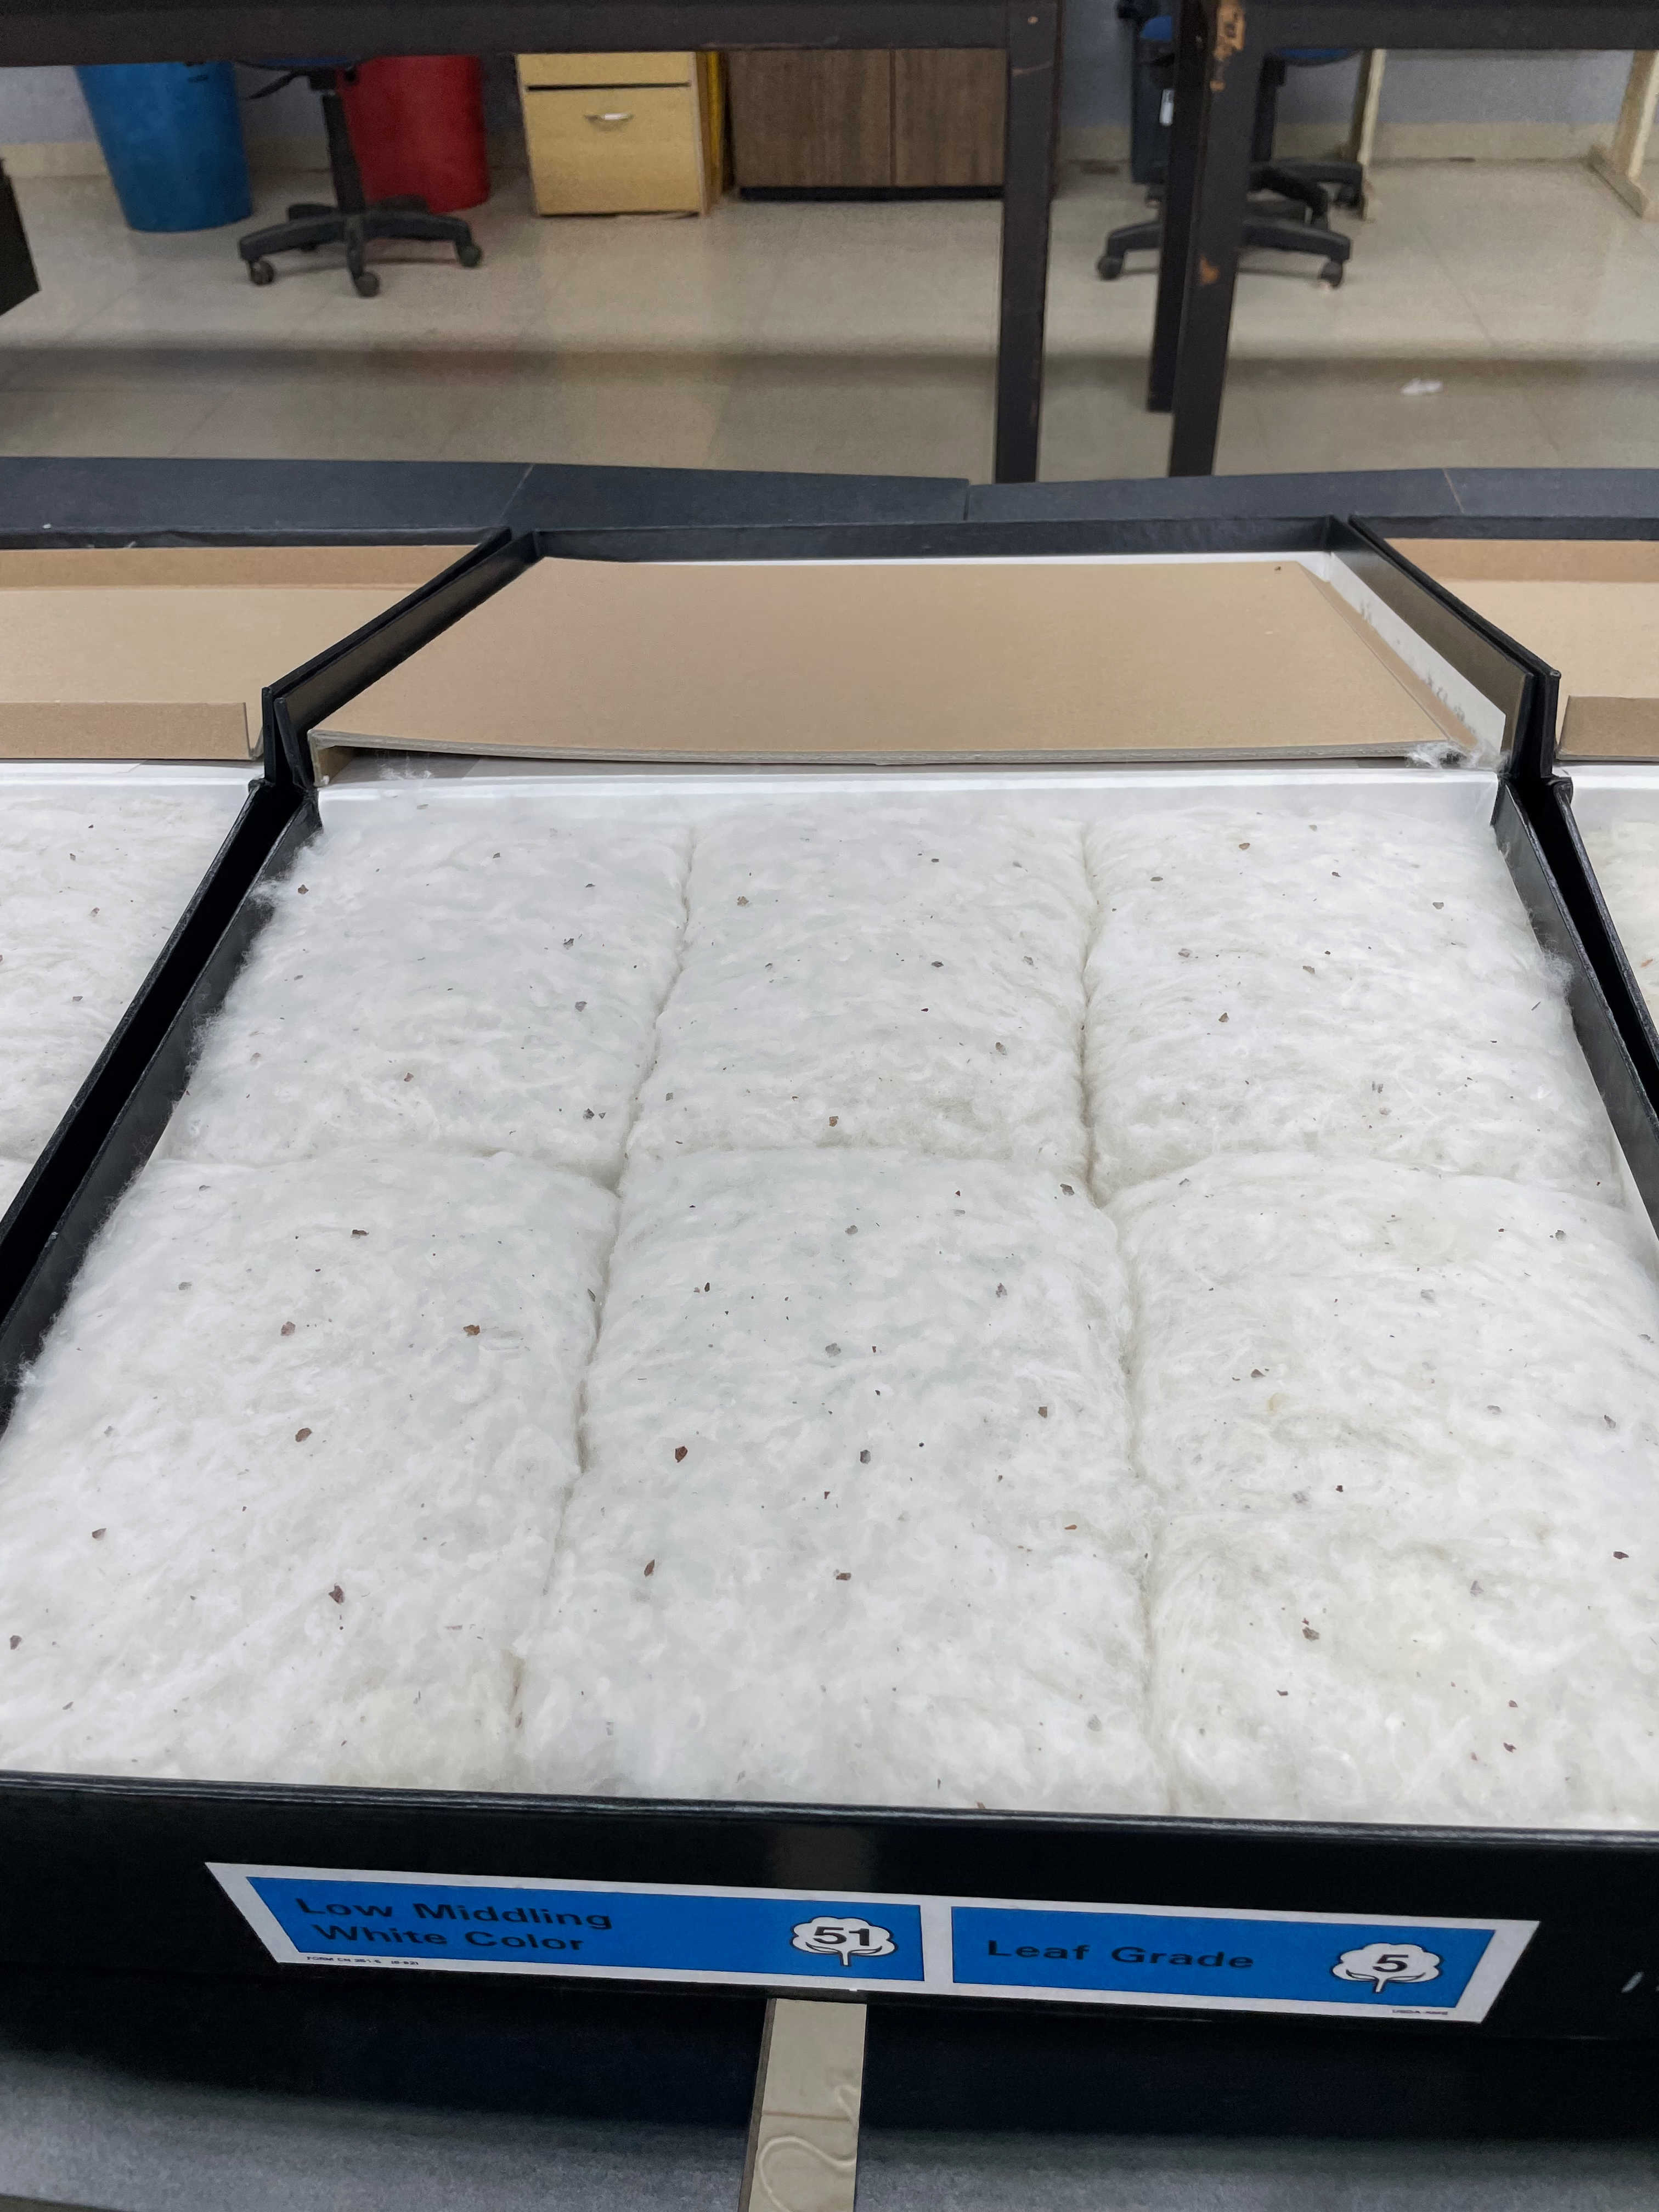
\includegraphics[trim={0 0 0 5cm},clip, scale=.3]{images/padrao_fisico_universal.jpeg}
	\end{center}
	\caption*{Fonte: Do Autor}
\end{figure}

O algodão é classificado em tipos de cor, representados por códigos que correspondem aos Padrões Físicos Universais, conforme apresentado na Tabela \ref{tab_tipo_cor} e por grau de folhas, conforme Tabela \ref{tab_grau_folha}.

Os procedimentos manuais para classificação visual são:

\begin{itemize}
    \item Visualizar os Padrões Físicos Universais antes de cada período de trabalho, a fim de memorizá-los e consultá-los, sempre que for necessário, podendo colocar a amostra de trabalho lado a lado dos Padrões Físicos;
    \item As caixas dos Padrões Físicos devem sempre estar fechadas e serem abertas somente no momento da visualização, além de estarem dentro do prazo de validade ; 
    \item Dividir no sentido longitudinal cada amostra ao meio, subdividindo as metades, tendo o cuidado de não descaracterizá-las durante o manuseio;
    \item Selecionar visualmente as duas piores partes (com as características de menor qualidade);
    \item Unir as quatro partes, deixando as duas piores nas faces externas, sendo a pior voltada para cima, definindo o grau de cor e de folha sempre em função da pior parte;
    \item Analisar visualmente as superfícies de cada amostra quanto à cor, brilho, manchas, conteúdo e tamanho das impureza, contaminações por matérias estranhas e defeitos de beneficiamento, seguindos os Padrões Físicos Universais;
    \item Selecionar as amostras por grupos semelhantes para facilitar o processo visual;
    \item Determinar o tipo do algodão com base nos códigos universais;
    \item Caso a amostra não se enquadre em nenhum Padrão Físico Universal, deve ser classificada como Fora de Tipo;
    \item Registrar o resultado da classificação em um Laudo de Classificação;
\end{itemize}

\afterpage{%
    \clearpage% Flush earlier floats (otherwise order might not be correct)
    \thispagestyle{empty}% empty page style (?)
    \begin{landscape}% Landscape page
        \centering % Center table
        \begin{table}
            \centering
            \caption{Códigos dos tipos de Cor, Classes de Cor ou Grau de Cor do Algodão Upland}
            \begin{tblr}{
                width = \linewidth,
                colspec = {Q[l,m,400]Q[c,m,180]Q[c,m,220]Q[c,m,180]Q[c,m,220]Q[c,m,180]},
                row{1} = {font=\bfseries},
                vline{2-6} = {-}{},
                hline{3-9} = {-}{},
                hline{1-2,10} = {2pt}
              }
                                                                                  & Branco & Ligeiramente Creme & Creme & Avermelhado & Amarelado \\
              Cor Boa Média - GM (Good Middling)                         & 11              & 12                          & 13             & -                    & -                  \\
              Cor Estritamente Média-SM (Strict Middling)                & 21              & 22                          & 23             & 24                   & 25                 \\
              Cor Média-M (Middling)                                     & 31              & 32                          & 33             & 34                   & 35                 \\
              Cor Estritamente Abaixo da Média-SLM (Strict Low Middling) & 41              & 42                          & 43             & 44                   & -                  \\
              Cor Abaixo da Média-LM (Low Middling)                      & 51              & 52                          & 53             & 54                   & -                  \\
              Cor Estritamente Boa Comum-SGO (Strict Good Ordinary)      & 61              & 62                          & 63             & -                    & -                  \\
              Cor Boa Comum-GO (Good Ordinary)                           & 71              & -                           & -              & -                    & -                  \\
              Abaixo de Padrão                                           & 81              & 82                          & 83             & 84                   & 85                 
              \end{tblr}
        \label{tab_tipo_cor}
        \end{table}
    \end{landscape}
    \clearpage
}
\begin{table}
    \centering
    \caption{Códigos dos Graus de Folha do Algodão Upland}
    \begin{tblr}{
        colspec = {Q[c,m]},
        row{1} = {font=\bfseries},
        hline{1-2,10} = {2pt}
        }
        Grau de Folha \\
        1                      \\
        2                      \\
        3                      \\
        4                      \\
        5                      \\
        6                      \\
        7                      \\                
        8                      \\    
    \end{tblr}
\label{tab_grau_folha}
\end{table}


\bibliography{bibliografia.bib} 

\end{document}